\chapter{Model Characterization} \label{chapter-characterization}


\section{Base model of city and the production sector}
\newpage
 \subsection{The price. of output}
Underlying the housing analysis is an economic model of the city including firms and transportation.  The first question for an economist is likely to be is, "Does the system respond to an increase in demand for its export product in the expected ways?" 


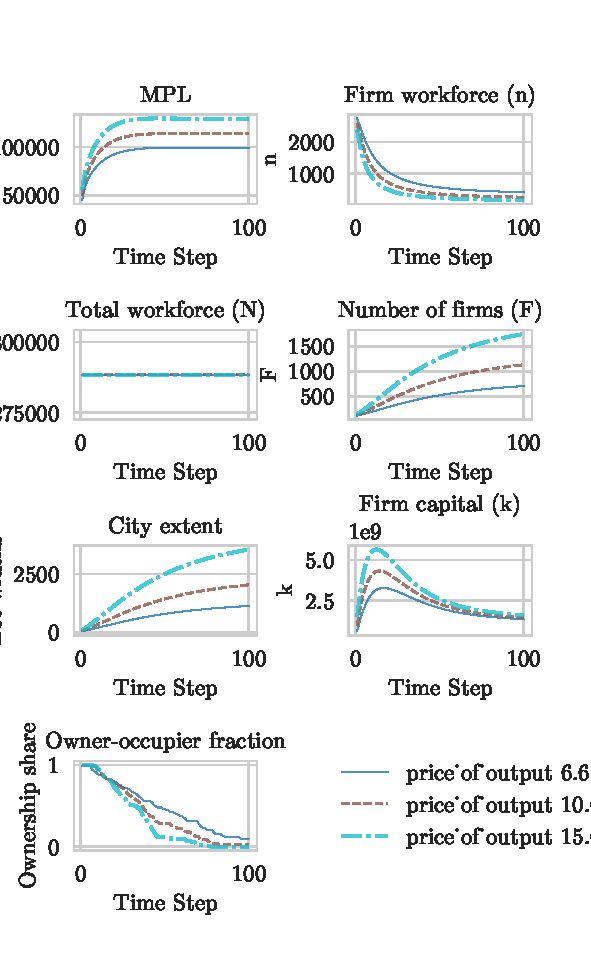
\includegraphics[scale=1]{fig/Analysis/price3.pdf}


 % \subsection{Change junk}
\begin{figure}
  \centering
  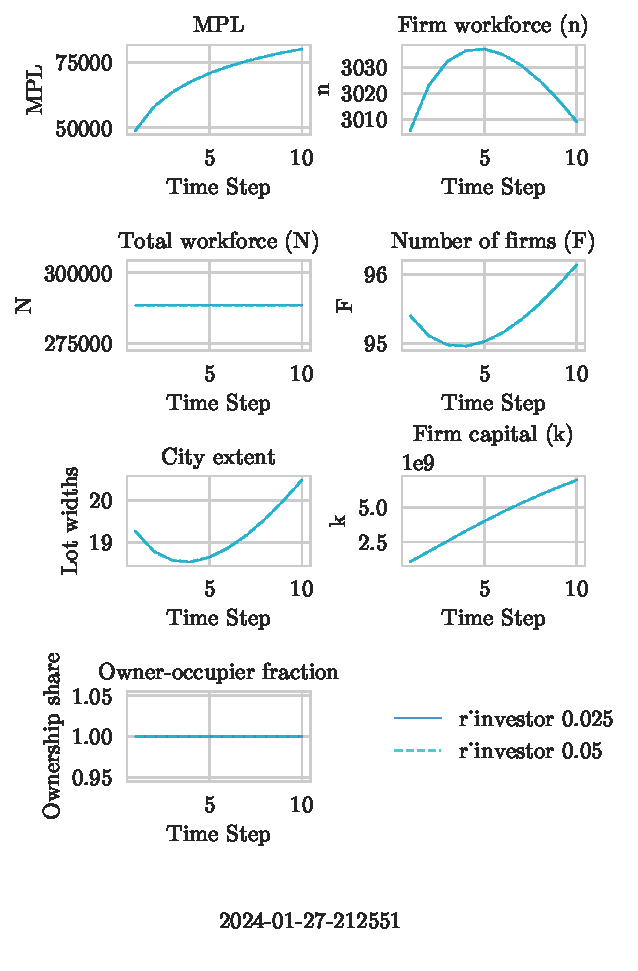
\includegraphics[width=.6\textwidth, clip, trim=0 20mm 0 0]{fig/plots/timeseries-plots-2024-01-27-212551.pdf}
  \caption{Your caption here.}
  \label{fig:your-label}
\end{figure}

 \subsection{Change Density}
 This experiment verifies that the labour-market/urban model that is the platform for the housing market analysis behaves exactly as expected when density changes. mpl, n, N, F, E, and k all rise. %Population rises with 

 The fraction owner-occupiers falls earlier with increasing density due to more rapid financialization and the potential rent capture increases, and not to changing housing form. It seems later entrants do not purchase. The transition is achieved in about two full generations in our model. The timing will be sensitive to the specific parameterization.
 

 \hspace*{-2cm}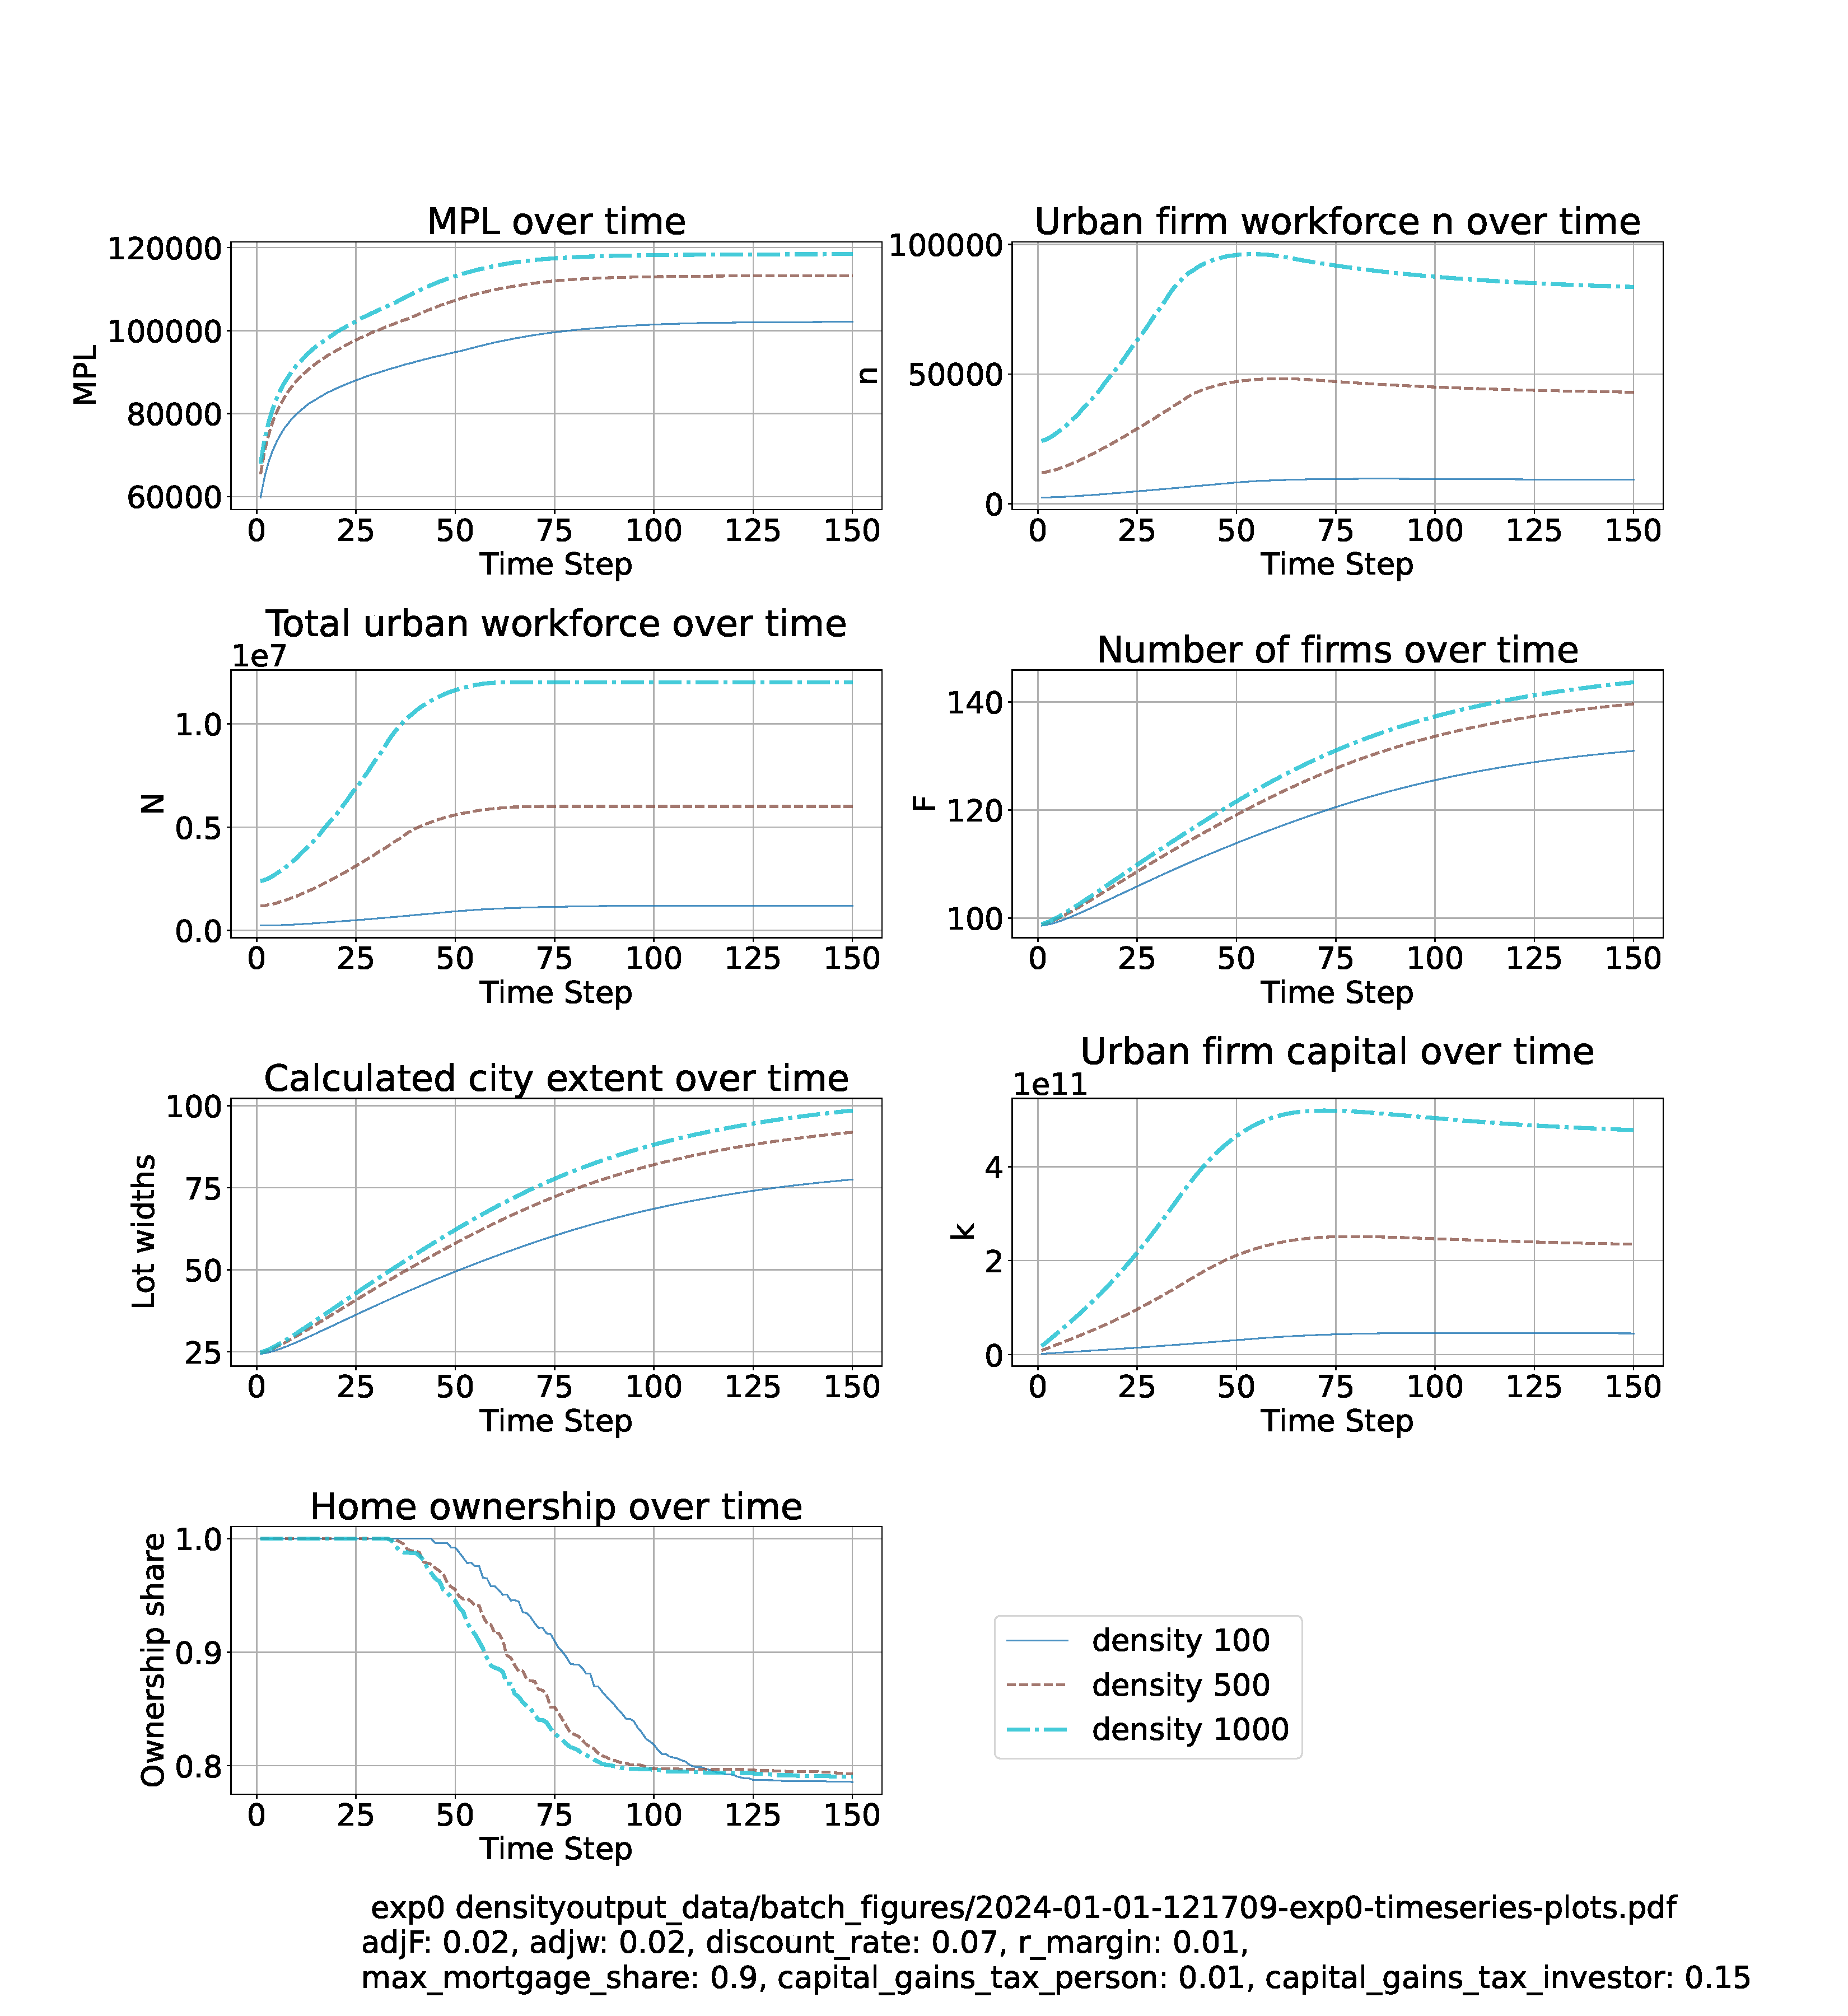
\includegraphics[trim= 1.5cm 3.65cm 2cm 4.0cm, clip, scale=.3]{fig/Analysis/Density-3-150.pdf}

\newpage %%%%%%%%%%%%%%%%%%%%%%%%%%%%%%%%%%

\subsection{High Gamma}
Very high levels of the agglomeration parameter Gamma are implausible. They drive up marginal productivity, causing very rapid growth, drive down firm size because the first worker is extremely productive but the MPL falls rapidly. Very small firms with high levels of capital multiply. Rapidly rising prices encourage investors while savings-limited owner-occupiers are squeezed out.

Higher agglomeration effects make land rents higher and increase the gains to investors, resulting in more rapid financialization of the housing stock.

%   we can check
 
% \begin{tabular}{|c|c||c|c||c|c|}
% mpl  & up   & n   & up & N   &  up \\
% F    & up   & E   &  up  &  k & up
% \end{tabular} 

 \hspace*{-2.5cm}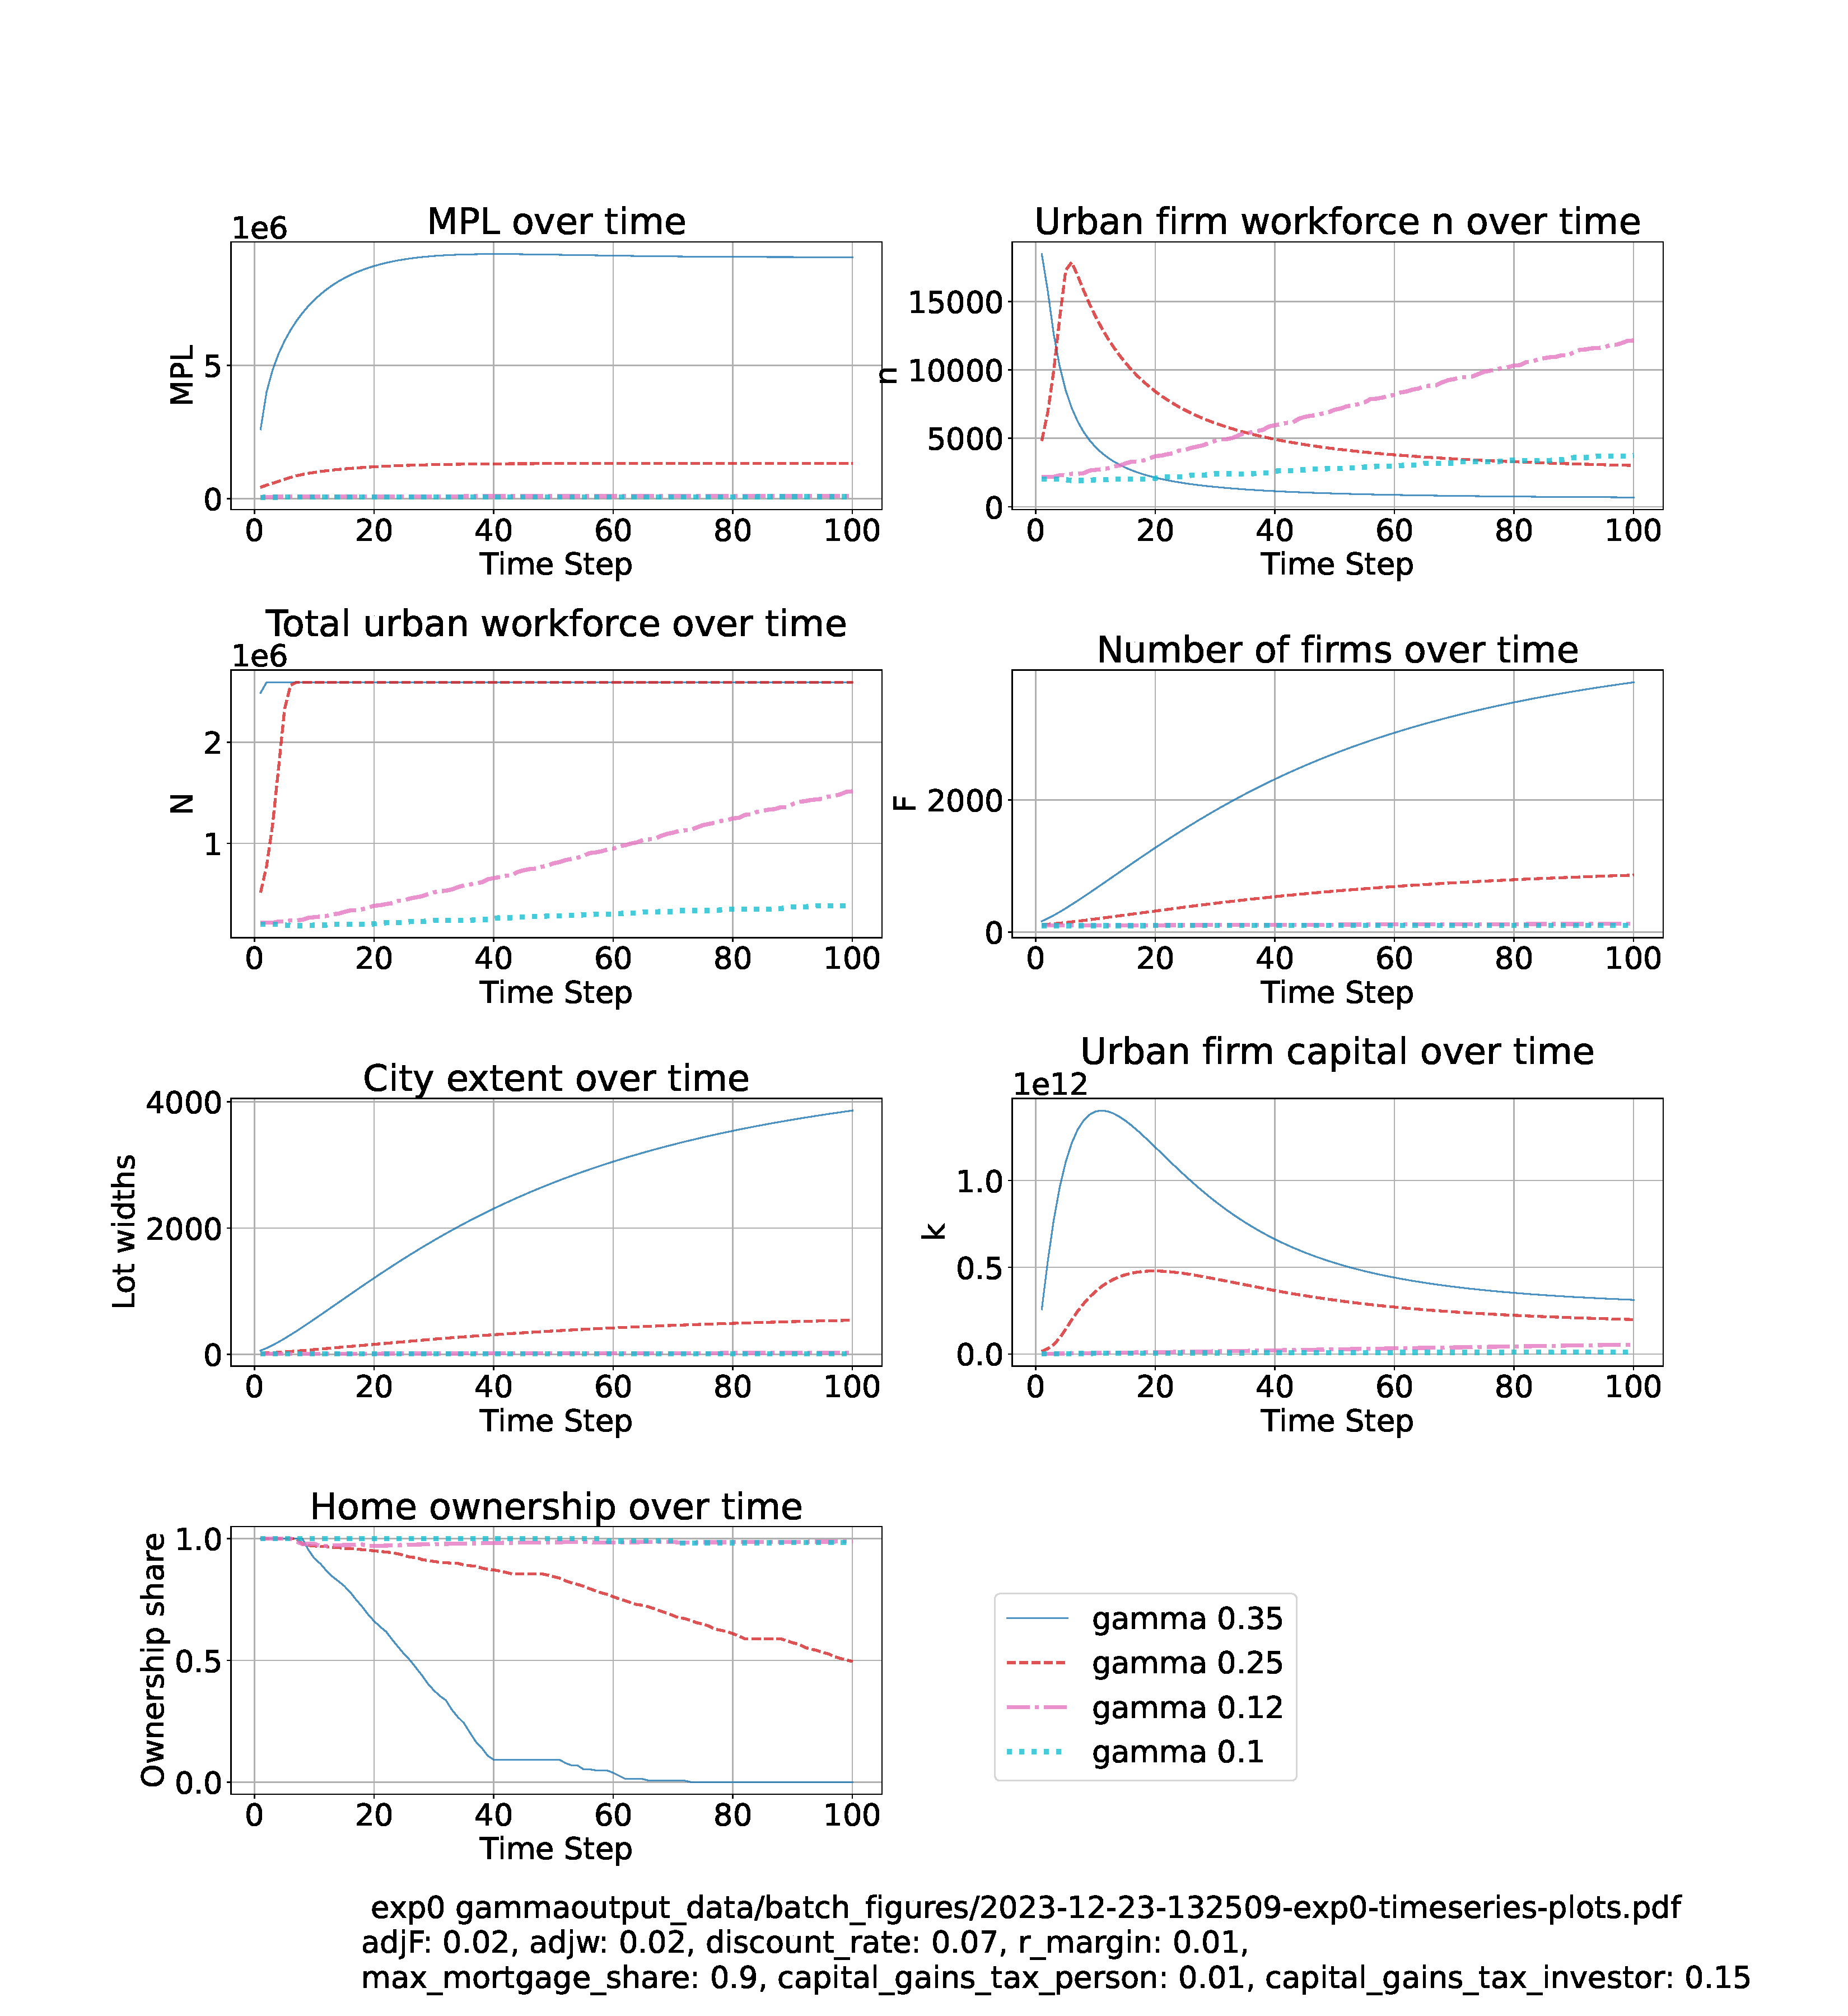
\includegraphics[trim= 1.5cm 3.65cm 2cm 4.0cm, clip, scale=.28]{fig/Analysis/Gamma-5-30.pdf}


\section{Investors can sell property}
We recognize that, like any other class of agents, investors vary in capacity, motive, information, and resources. For conceptual an computational simplicity we nonetheless treat investors a single agent making multiple purchases and holding multiple properties.\footnote{There is a conceptual issue just beneath the surface here: are we concerned with the class of investors as individuals or are the individuals simply the channels through which an abstract quantity called financial capital works? We do not engage this debate, but we note that our project is to describe the effect of financial capital, not individual investors. Our modelling of the process is implicitly consistent with analyses that treat capital as an  conceptual entity rather than as a conceptual fiction that is convenient for discussing the aggregate outcomes of individual behaviours. }

Even so it is good theoretical practice to ensure that the representative agent's behaviour is consistent with plausible individual investor motives and actions.\footnote{This appears to be the common practice in economics, where modeling decisions about aggregate variables like prices, quantities, investment, employment are supported by stories about individual decisions.} 

Since investors both buy and sell properties, for example, we make a share of the investor's properties available to the market in each period. This fraction, say 5 percent, is made available for potential homeowners as well as for repurchase (nominally by other investors). We can vary this fraction in response to capital market conditions, the tax regime, legislation, and the state of investor expectations. Small changes in invest of confidence might have significant effect of prices in the sort run, while persistent changes are likely to change the ownership pattern in the city. This device retains the simplicity we want while allowing for a range of shocks and interventions to influence the market.

We simplify the computation by comparing the reservation price of the investor for the randomly selected properties with the bid of the richest newcomer. If there is no newcomer able to beat the reservation price of the investor, we assume any exchange of properties will be between investors. No investment properties enter the market in that period. 

\section{General behaviour of the model with a price shock}


Figure~\ref{fig:enter-label} illustrates a number of features of the way firms, population and city size evolve for a specific parameterization. %This sub-model serves as the economic platform for our study of the housing market. Parameters have been chosen to produce a plausible pattern of development.
We consider a 20\% drop in  the price of the city's output. The decline in demand for the city's output will normally affect the overall demand for labour, individual firm employment $n$, the number of firms $F$, and the size of the city. The time paths are interrelated and depend on adjustment speeds for each variable. Some  adjustment speeds are restricted  for this illustration.

The upper left panel in Figure~\ref{fig:enter-label} shows the evolution of the urban wage  in red. The pattern of wage growth shown by the solid thin line  is due to the growing agglomeration effect over time. In this illustrative case, the wage adjusts with no lag. The sharp dip in the thick  line shows the wage responding immediately to the change in demand conditions, followed by a return to a path slightly below the no-shock level,  eventually converging to the original path. 


With the parameter set illustrated, firm employment shown in the middle left, does not fall noticeably in the face of the price shock because the wage adjusts immediately.  Since firm size does not fall, the number of firms, shown in the lower right must fall, and it does. Entry and exit takes time, so the number of firm responds with a lag. 
The middle right panel shows the effect  on aggregate demand and supply for labour. Both fall and are sow to recover. Aggregate labour demand in red adjusts slowly but supply responds immediately because city size, shown in the lower left,  has been allowed to adjust instantly. Realistically, population and city size adjust slowly, and the actual path would depend on the adjustment rates.

The upper right shows a more protracted effect on the individual firm's capital accumulation simply because capital can be adjusted more slowly than labour. 

